%==============================================================================
%  DRAFT -- IEEE Wireless Communications Letters style
%  Revised to align the formulation and MAML discussion with the reference
%  RIS-NOMA and RIS-ISAC papers while keeping the present simulation results.
%==============================================================================
\documentclass[10pt,journal]{IEEEtran}

\usepackage{graphicx}
\usepackage{epstopdf}
\usepackage{amsmath}
\usepackage{newtxtext,newtxmath}
\usepackage{bm}
\usepackage{booktabs}
\usepackage{url}
\usepackage[caption=false,font=footnotesize]{subfig}
\usepackage[ruled,vlined]{algorithm2e}
\usepackage{tikz}
\usepackage{pgfplots}
\pgfplotsset{compat=1.18}
\usetikzlibrary{arrows.meta,shapes.geometric,positioning}

\graphicspath{{figs/}}
\DeclareGraphicsExtensions{.pdf,.eps,.png,.jpg,.jpeg}

\newcommand{\Rdl}{R_{\mathrm{DL}}}
\newcommand{\Rsum}{R_{\mathrm{sum}}}
\newcommand{\bh}{\bm{h}}
\newcommand{\bw}{\bm{w}}
\newcommand{\bG}{\bm{G}}
\newcommand{\bH}{\bm{H}}
\newcommand{\bA}{\bm{A}}
\newcommand{\bPhi}{\bm{\Phi}}
\newcommand{\herm}{^{\mathsf{H}}}
\newcommand{\Cset}{\mathbb{C}}
\newcommand{\Eset}{\mathbb{E}}

\begin{document}

\title{Meta-Learning-Driven Joint Power Allocation and Phase-Shift Design
for RIS-Assisted NOMA-ISAC Systems}

% >>> PLACEHOLDER author block
\author{First~Author,~\IEEEmembership{Graduate~Student~Member,~IEEE,}
        Second~Author,~\IEEEmembership{Member,~IEEE,}
        and Third~Author,~\IEEEmembership{Senior~Member,~IEEE}
\thanks{Manuscript received \ldots; revised \ldots. This work was supported in
part by \ldots. \emph{(Corresponding author: First Author.)}}
\thanks{The authors are with the \ldots, \ldots\ (e-mail: author@univ.edu).}}

\markboth{IEEE Wireless Communications Letters,~Vol.~XX, No.~X, Month~2026}%
{Author \MakeLowercase{\textit{et al.}}: Meta-Learning-Driven Joint Power and Phase Design for RIS-Assisted NOMA-ISAC}

\maketitle

%==============================================================================
\begin{abstract}
This letter investigates a reconfigurable intelligent surface (RIS)-assisted
multiple-input single-output (MISO) integrated sensing and communication (ISAC)
system, where a base station (BS) simultaneously serves a near and a far user
via non-orthogonal multiple access (NOMA) while illuminating a sensing target.
We maximize a weighted communication-and-sensing throughput by jointly
optimizing the NOMA power-allocation coefficients and the RIS phase shifts,
subject to an aggregate communication QoS floor, individual near/far-user QoS
floors, and a sensing QoS constraint. To tackle the resulting non-convex problem,
a model-agnostic meta-learning (MAML)-based deep-learning algorithm is proposed.
A lightweight network predicts the low-dimensional power split, while an inner
optimizer adapts the high-dimensional RIS phase vector for each channel
realization. A first-order meta-update then trains the power map using the
phase-adapted channels, avoiding the unstable higher-order derivatives observed
in this high-SINR setting. Simulation results show
stable convergence, a strong RIS-aperture gain, and consistent improvements
against OMA, no-RIS, and partially optimized baselines.
\end{abstract}

\begin{IEEEkeywords}
Reconfigurable intelligent surface (RIS), integrated sensing and communication
(ISAC), non-orthogonal multiple access (NOMA), deep learning, meta-learning
(MAML), MISO.
\end{IEEEkeywords}

%==============================================================================
\section{Introduction}
\IEEEPARstart{I}{ntegrated} sensing and communication (ISAC) has emerged as a
key enabler for next-generation wireless networks, jointly designing sensing
and communication on a shared spectral and spatial resource to improve
spectrum, energy, and hardware efficiency~\cite{liu2022isac,deng2025mmwave}.
When combined with NOMA, which superposes users in the power domain and
separates them by successive interference cancellation (SIC), ISAC can further
raise spectral efficiency. Severe blockage and path loss, however, degrade both
functions, motivating the use of an RIS to reshape the propagation environment
through low-cost passive elements~\cite{wu2020ris}.

RIS-assisted ISAC resource management has attracted growing interest. In
\cite{wang2025hybrid}, hybrid beamforming and RIS phase shifts were jointly
optimized to shape the ISAC beampattern. In \cite{lyu2024crb}, a penalty-based
block-coordinate method minimized the Cramer-Rao bound for RIS-aided mmWave
ISAC. A rate-splitting RIS-ISAC design was studied in \cite{ke2025rsma}. For
RIS-NOMA networks, \cite{zou2023ml} developed a DL/MAML framework that jointly
optimizes BS power allocation and RIS phase shifts. These results motivate a
learning-based factorization of the coupled phase-and-power design: the
low-dimensional power allocation is predicted by a neural network, whereas the
high-dimensional RIS phase is refined per channel realization.

The main contributions are summarized as follows. First, we formulate a
weighted communication-plus-sensing throughput maximization problem containing
both a cluster-level communication QoS floor and individual near/far-user QoS
floors, so aggregate spectral efficiency cannot hide user starvation. Second,
we develop a first-order MAML-based bilevel algorithm in which the power split
is predicted from the current phase-dependent channel features and the RIS phase
is adapted by a short per-channel inner optimization. Third, we discuss the
algorithmic convergence limitations and the offline/online computational cost,
and provide a reproducible simulation table containing the actual link
distances, fading/path-loss settings, RIS size, power, and learning parameters.

%==============================================================================
\section{System Model and Problem Formulation}

\begin{figure}[t]
\centering
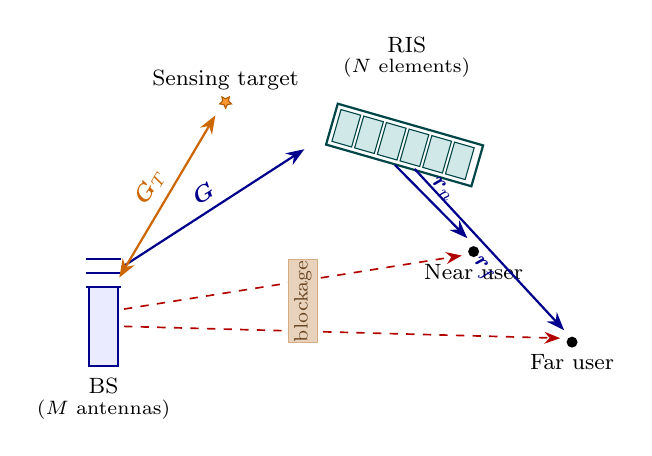
\begin{tikzpicture}[>=Stealth,font=\footnotesize,
  comm/.style={->,thick,blue!55!black},
  sens/.style={<->,thick,orange!80!black},
  block/.style={->,semithick,red!70!black,dashed}]
\filldraw[fill=blue!8,draw=blue!55!black,thick] (-0.18,0) rectangle (0.18,1.0);
\foreach \y in {1.0,1.18,1.36}{\draw[blue!55!black,thick] (-0.22,\y)--(0.22,\y);}
\node[align=center,below=1pt] at (0,0) {BS\\[-2pt]\scriptsize($M$ antennas)};
\begin{scope}[shift={(2.9,2.85)},rotate=-16]
  \foreach \i in {0,...,5}{\filldraw[fill=teal!18,draw=teal!55!black]
  (\i*0.30,0) rectangle (\i*0.30+0.26,0.42);}
  \draw[teal!55!black,thick] (-0.06,-0.06) rectangle (1.86,0.48);
\end{scope}
\node[align=center,above=1pt] at (3.85,3.5) {RIS\\[-2pt]\scriptsize($N$ elements)};
\node[circle,fill=black,inner sep=1.4pt] (un) at (4.7,1.45) {};
\node[below=1pt] at (un) {Near user};
\node[circle,fill=black,inner sep=1.4pt] (uf) at (5.95,0.3) {};
\node[below=1pt] at (uf) {Far user};
\node[star,star points=5,star point ratio=0.5,draw=orange!70!black,
      fill=orange!80,inner sep=1.6pt] (tg) at (1.55,3.35) {};
\node[above=1pt] at (tg) {Sensing target};
\draw[comm] (0.23,1.25) -- node[above,sloped]{$\bm{G}$} (2.55,2.75);
\draw[comm] (3.7,2.55) -- node[above,sloped]{$\bm{r}_n$} (4.62,1.62);
\draw[comm] (3.95,2.5) -- node[below,sloped,pos=0.55]{$\bm{r}_f$} (5.85,0.45);
\draw[sens] (0.2,1.12) -- node[above,sloped]{$\bm{G}_T$} (1.42,3.18);
\draw[block] (0.26,0.72) -- (4.55,1.4);
\draw[block] (0.26,0.5) -- (5.8,0.35);
\filldraw[fill=brown!35,draw=brown!65] (2.35,0.30) rectangle (2.72,1.35);
\node[rotate=90,brown!55!black] at (2.53,0.82) {\scriptsize blockage};
\end{tikzpicture}
\caption{System model: a MISO BS serves a near and a far user via NOMA with an
$N$-element RIS while sensing a point target.}
\label{fig:system}
\end{figure}

\subsection{System Model}
As illustrated in Fig.~\ref{fig:system}, a BS equipped with $M$ antennas serves
a single-antenna near user (n) and far user (f) and illuminates a point sensing
target (T). The RIS contains $N$ passive reflecting elements. Following the
standard RIS model in \cite{zou2023ml,wei2026ris}, the coefficient of element
$i$ is
\begin{equation}
 v_i=\beta_i e^{j\phi_i},\qquad 0\leq\beta_i\leq1,\quad \phi_i\in[0,2\pi),
\end{equation}
and
\begin{equation}
\bPhi=\mathrm{diag}(\beta_1e^{j\phi_1},\ldots,\beta_Ne^{j\phi_N}).
\end{equation}
For an ideal passive RIS we set $\beta_i=1$ for all $i$, as commonly adopted to
maximize reflected power~\cite{zou2023ml,wei2026ris}; hence only the phases are
optimized.

\subsubsection{Channel Model}
Let $\bG\in\Cset^{N\times M}$ denote the BS-RIS channel and
$\bm{r}_k\in\Cset^N$ the RIS-user channel. The cascaded channel of user
$k\in\{n,f\}$ is
\begin{equation}
\bh_k=\bG\herm\bPhi\bm{r}_k\in\Cset^M. \label{eq:cascade}
\end{equation}
All links use distance-dependent large-scale attenuation and small-scale fading.
In the RIS-aided case the direct BS-user links are blocked and
\eqref{eq:cascade} dominates; the no-RIS baseline retains only the weak direct
link. The round-trip sensing response is represented by
$\bG_T\in\Cset^{M\times M}$ and can be written for a point target as
\begin{equation}
\bG_T=\sqrt{\beta_T}(\bG\herm\bPhi\bm{h}_{TR})
(\bm{h}_{RT}\herm\bPhi\bG),
\end{equation}
where $\beta_T$ is the round-trip target/path gain (40 dB in the simulator) and
$\bm{h}_{RT}$ and $\bm{h}_{TR}$ denote the RIS-target and target-RIS links. This
rank-one sensing form and the use of transmit/receive beamformers are consistent
with RIS-assisted ISAC models such as \cite{wang2025hybrid,lyu2024crb}.

\subsubsection{NOMA Communication and Sensing Model}
The BS transmits
\begin{equation}
\bm{x}=\left(\sqrt{a_nP}s_n+\sqrt{a_fP}s_f\right)\bw_c
       +\sqrt{a_TP}\bw_Ts_T, \label{eq:tx}
\end{equation}
where $P$ is the total BS power and
$\bm{a}=[a_n,a_f,a_T]$ contains the near-user, far-user, and sensing power
fractions. The coefficients satisfy $a_n+a_f+a_T=1$ and $a_k\geq0$. The
beamforming vectors $\bw_c$ and $\bw_T$ are unit-norm communication and sensing
beamformers, respectively. Beamforming notation of this form is standard in
RIS-ISAC resource allocation~\cite{wang2025hybrid,wei2026ris}.

For power-domain NOMA, both users share the common beam $\bw_c$ and are
separated by SIC~\cite{zou2023ml,sun2024noma}. In the implemented fair-NOMA
configuration, the communication beam is a normalized weighted combination
\begin{equation}
\bw_c=\frac{0.7\bh_f+0.3\bh_n}{\|0.7\bh_f+0.3\bh_n\|}, \label{eq:wc}
\end{equation}
which deliberately gives the weaker far user the larger steering weight while
retaining near-user gain. The symbols $\bw_c$ and $\bw_T$ therefore denote
unit-norm active transmit beamforming vectors at the BS, whereas $\beta_i$ is
the passive amplitude coefficient of RIS element $i$; these quantities play
different roles and should not be conflated. Beamforming/RIS notation of this
form is standard in RIS-NOMA/ISAC models~\cite{zou2023ml,wang2025hybrid}.

For sensing, define $\bH_u=[\bh_n,\bh_f]$. The implemented sensing beam is the
dominant eigenvector of the leakage-penalized Hermitian matrix
\begin{equation}
